% Parte 1: Introdução
\section{Introdução à Evolução}

\begin{frame}{Linha do Tempo das Redes Móveis}
\begin{columns}
    \begin{column}{0.45\textwidth}
        \begin{itemize}
            \item 1G: Voz analógica
            \item 2G: Digital, SMS
            \item 3G: Dados móveis iniciais
            \item 4G: LTE, banda larga IP
            \item 5G: eMBB, mMTC, URLLC
        \end{itemize}        
    \end{column}
    \begin{column}{0.55\textwidth}
        \vspace{1cm}
        \begin{figure}
            \centering
            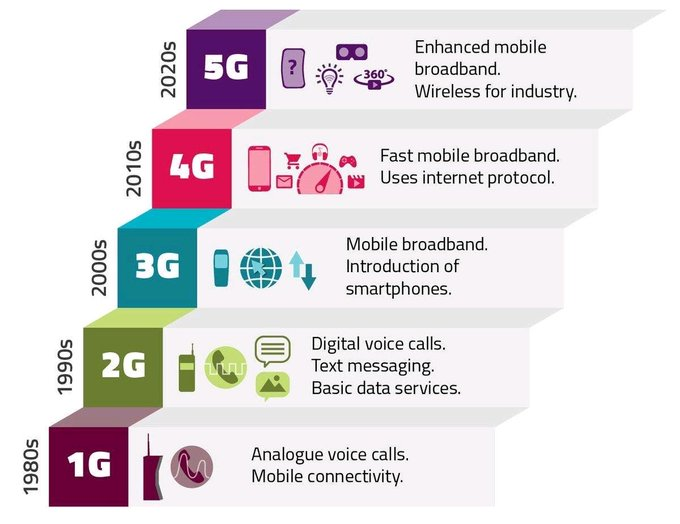
\includegraphics[width=\linewidth]{figs/Network-Generation-Progression.jpg}
            \caption{Telefonia móvel\footnote{\href{https://galooli.com/glossary/what-is-a-network-generation/}{https://galooli.com/glossary/what-is-a-network-generation/}}}
            \label{fig:placeholder}
        \end{figure}
    \end{column}
\end{columns}

\end{frame}

\begin{frame}{Tendências Tecnológicas}
\begin{itemize}
  \item Mais banda e menor latência
  \begin{itemize}
    \item \textbf{Largura de banda ampliada}: suporte a taxas de dezenas de Gbps com novas faixas de espectro, incluindo ondas milimétricas.  
    \item \textbf{Redução da latência}: níveis próximos de 1 ms, viabilizando aplicações em tempo real.  
    \item \textbf{Impacto prático}: telemedicina (cirurgias remotas), realidade virtual imersiva, controle de sistemas industriais críticos.  
  \end{itemize}
  \item Maior densidade de dispositivos
  \begin{itemize}
    \item \textbf{Crescimento exponencial}: milhões de dispositivos conectados% (/km²).  
    \item \textbf{Soluções tecnológicas}: massive MIMO, beamforming e uso de small cells.  
    \item \textbf{Cenários típicos}: centros urbanos, estádios, fábricas inteligentes e ambientes de alta concentração populacional.  
    \item \textbf{Desafio}: garantir eficiência energética e escalabilidade sem perda de qualidade de serviço.  
  \end{itemize}
  % \item Casos de uso: IoT, RA, veículos conectados
\end{itemize}
\end{frame}

\begin{frame}{Casos de uso emergentes}
\begin{itemize}
  \item \textbf{IoT (Internet das Coisas)}: suporte a bilhões de sensores e atuadores, baixo consumo de energia, comunicações massivas e esporádicas.  
  \item \textbf{Realidade Aumentada (RA)}: necessidade de sincronização imediata entre mundo físico e digital, alta taxa de transmissão e baixíssima latência.  
  \item \textbf{Veículos conectados (V2X)}: comunicações ultraconfiáveis para navegação segura, prevenção de acidentes e coordenação entre veículos autônomos.  
  \item \textbf{Visão futura}: redes adaptáveis e programáveis que suportem simultaneamente diferentes requisitos de QoS.  
\end{itemize}
\end{frame}

\begin{frame}
    \frametitle{Arquitetura do 5G}
    \begin{itemize}
        \item \textbf{Rede de Acesso por Rádio (RAN)}: Nova radiofrequência e técnicas avançadas de transmissão.
        \item \textbf{Rede Central (Core)}: Baseada em software, mais flexível e ágil.
        \item \textbf{Suporte Multisserviço}: \textit{Network slicing} para diferentes tipos de serviços.
    \end{itemize}
    \begin{figure}
        \centering
        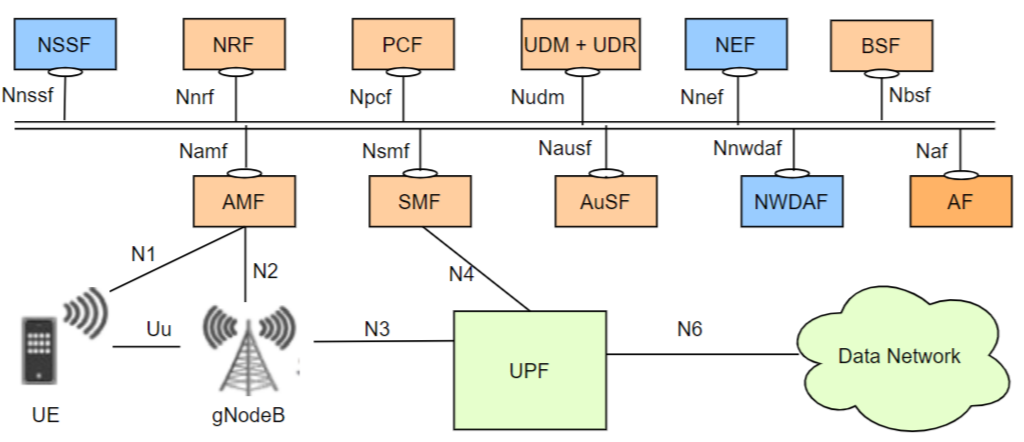
\includegraphics[width=0.7\textwidth]{figs/ArquiteturaGeral5G}
        \caption{Arquitetura Geral do 5G\footcite{5G_architecture}}
    \end{figure}
    \vspace{0.4cm}
\end{frame}

\begin{frame}
    \frametitle{Características Técnicas do 5G}
    \begin{itemize}
        \item \textbf{Velocidade}: Até 20 Gbps.
        \item \textbf{Latência}: Menos de 1 ms.
        \item \textbf{Conectividade Massiva}: Suporte para até 1 milhão de dispositivos por km².
        \item \textbf{Eficiência Espectral}: Utilização otimizada do espectro.
    \end{itemize}
    \begin{figure}
        \centering
        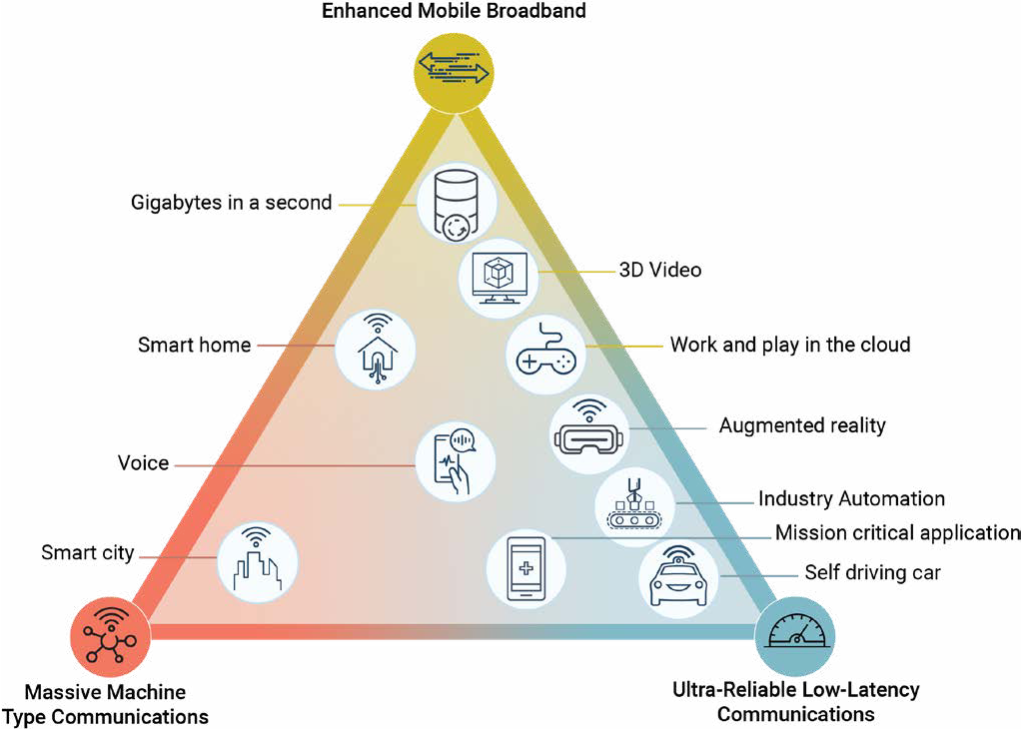
\includegraphics[width=0.5\linewidth]{figs/5G_verticais.png}
        \caption{Requisitos para diferentes tipos de aplicações\footnote{\href{https://www.cio.gov/assets/files/Framework-to-Conduct-5G-Testing-508.pdf}{https://www.cio.gov/assets/files/Framework-to-Conduct-5G-Testing-508.pdf}}}
    \end{figure}
\end{frame}